\documentclass[xcolor=dvipsnames]{beamer}
\useoutertheme{infolines}
\setbeamertemplate{navigation symbols}{}
\setbeamertemplate{items}[ball]
\usepackage{graphicx,multirow,color,xcolor,verbatim,float,comment,amsmath}
\setbeamertemplate{frametitle}[default][center]
\begin{document}
\title{Parameter Selection on Simultaneous Driver Pathway Detection}
\author{Bowen Deng}
\institute{Dept. of Prob. and Stat.}
\date{}
\begin{frame}
\maketitle
\end{frame}
\begin{frame}
\tableofcontents
\end{frame}
\section{Review}
\begin{frame}{Background}
Our objective is to identify multiple driver mutation pathways in cancer genes based on the mutation data matrix.\\
The problem is available after the assumption that driver mutation pathways enjoy two blessings:\\
\begin{itemize}
\item Coverage: Almost every patient has at least one mutation in the pathway.\\
\item Exclusivity: Almost every patient has exactly one mutation in the pathway.\\
\end{itemize}
\end{frame}
\begin{frame}{Motivation}
View the problem as the maximization of De Novo submatrix score, i.e., $S(M)=\sum_{i=1}^m(1-|r_i-1|)$, where $r_i$ is the i-th row sum of $M$.\\
To identify $t$ mutually exclusive driver pathways, we want to maximize $\sum_{\rho=1}^tS(M_{\rho})$.\\
The problem is equivalent to a Binary Linear Programming task:\\
\begin{displaymath}
\begin{split}
\max O(M_1,\cdots,M_t)=\sum_{\rho=1}^t\sum_{i=1}^m(2C_i(M_{\rho})&-\sum_{j=1}^nI_{M_{\rho}}(j)A_{ij})\\
s.t. \sum_{j=1}^nI_{M_{\rho}}(j)A_{ij}&\geqslant C_i(M_{\rho})\\
\sum_{\rho=1}^tI_{M_{\rho}}(j)&\leqslant 1\\
\end{split}
\end{displaymath}
\end{frame}
\section{Selection of Parameters}
\begin{frame}{Selection of High Score Threshold}
For fixed parameter, we set up a high score threshold $s_0$, a gene pathway $M$ is good if $S(M)>s_0$.\\
$s_0$ is selected with permutation test.\\
We shuffle the mutation matrix $A$ by per row.\\
\begin{figure}
\centering
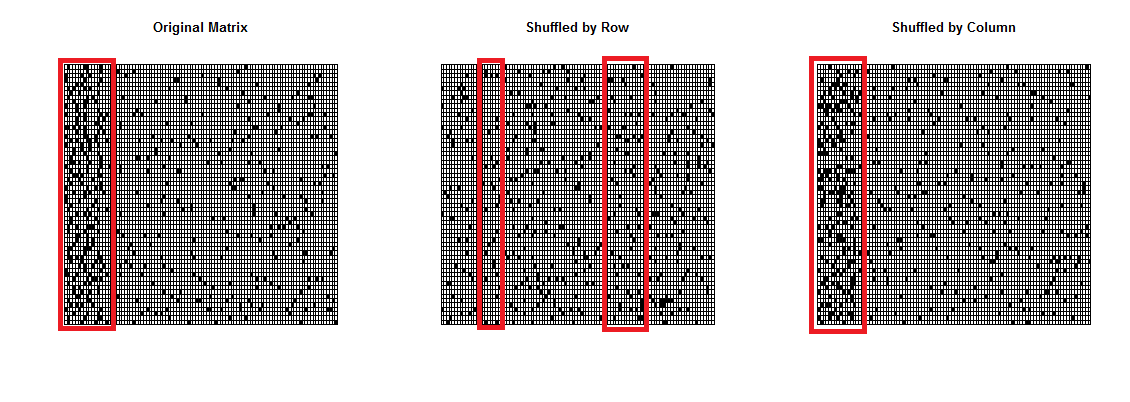
\includegraphics[width=0.99\linewidth]{shuffle.png}
\caption{The comparison of different shuffling strategies}
\end{figure}
\end{frame}
\begin{frame}
We assume that for the appropriate parameters, the score of the original mutation matrix is larger than it of the shuffled matrices.\\
\begin{figure}
\centering
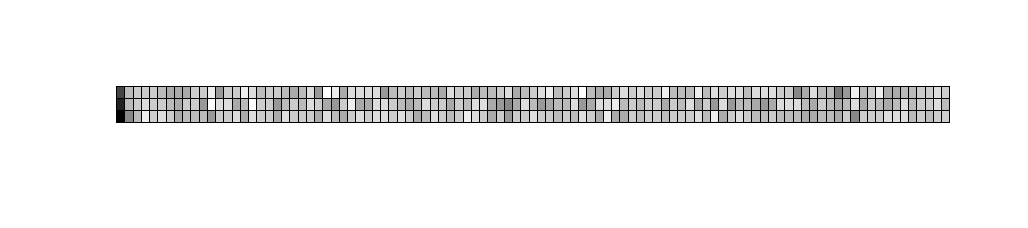
\includegraphics[width=0.99\linewidth]{permint.png}
\caption{Score Pattern with exact parameters: $t=3$, $4\leqslant k\leqslant 6$, the first column represents score of pathways in original data matrix, the others represent the scores of shuffled matrices}
\end{figure}
\end{frame}
\section{Numerical Results}
\begin{frame}
We simulate data matrix $A$ ($50\times 100$) with three pathways: $1-6$, $7-10$, $11-16$.\\
With MDendrix, the scores of the three detected pathways are 38, 46, 42, the sum of scores is 126.\\
\begin{figure}
\centering
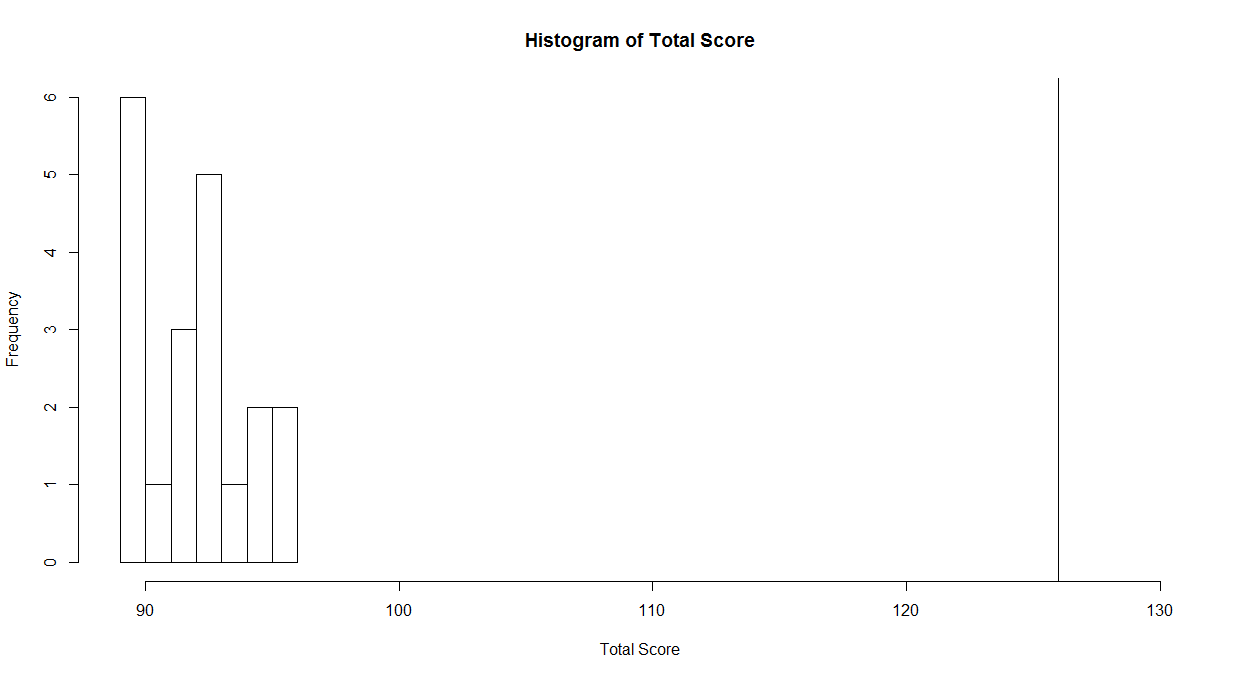
\includegraphics[width=0.9\linewidth]{histrow.png}
\caption{Histogram of Total Score, matrices are permuted by row}
\end{figure}
\end{frame}
\begin{frame}
\begin{figure}
\centering
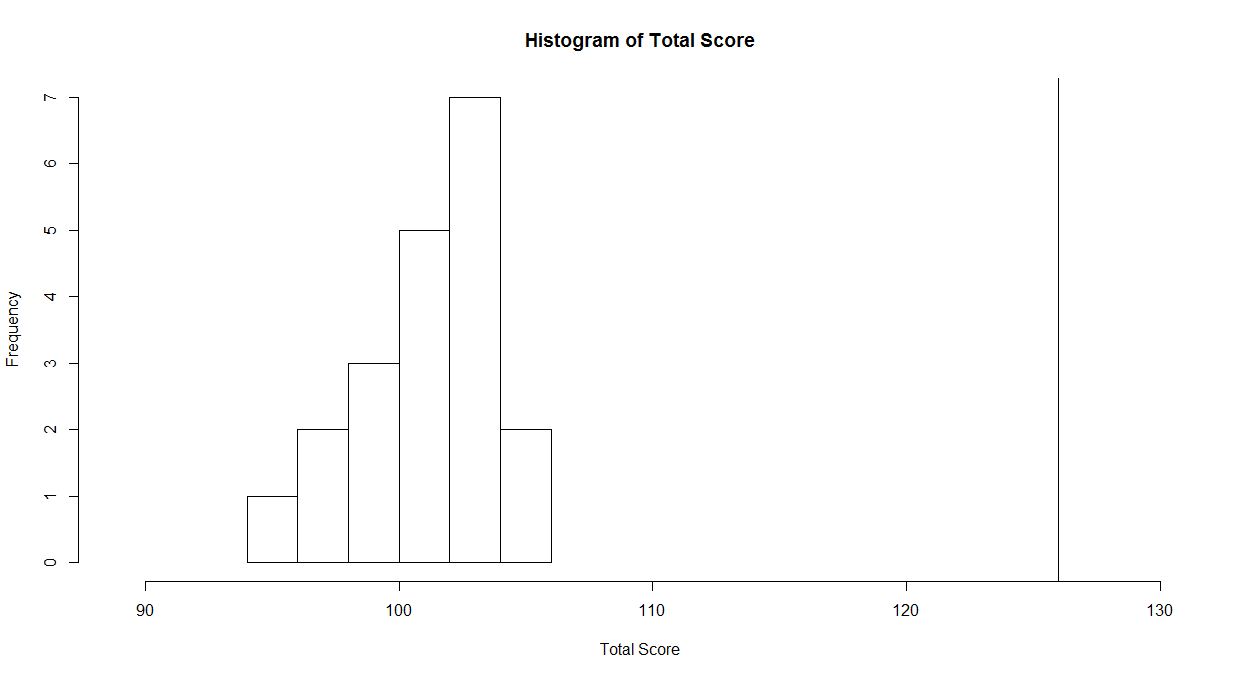
\includegraphics[width=0.9\linewidth]{histcol.png}
\caption{Histogram of Total Score, matrices are permuted by column}
\end{figure}
\end{frame}
\begin{frame}
\begin{figure}
\centering
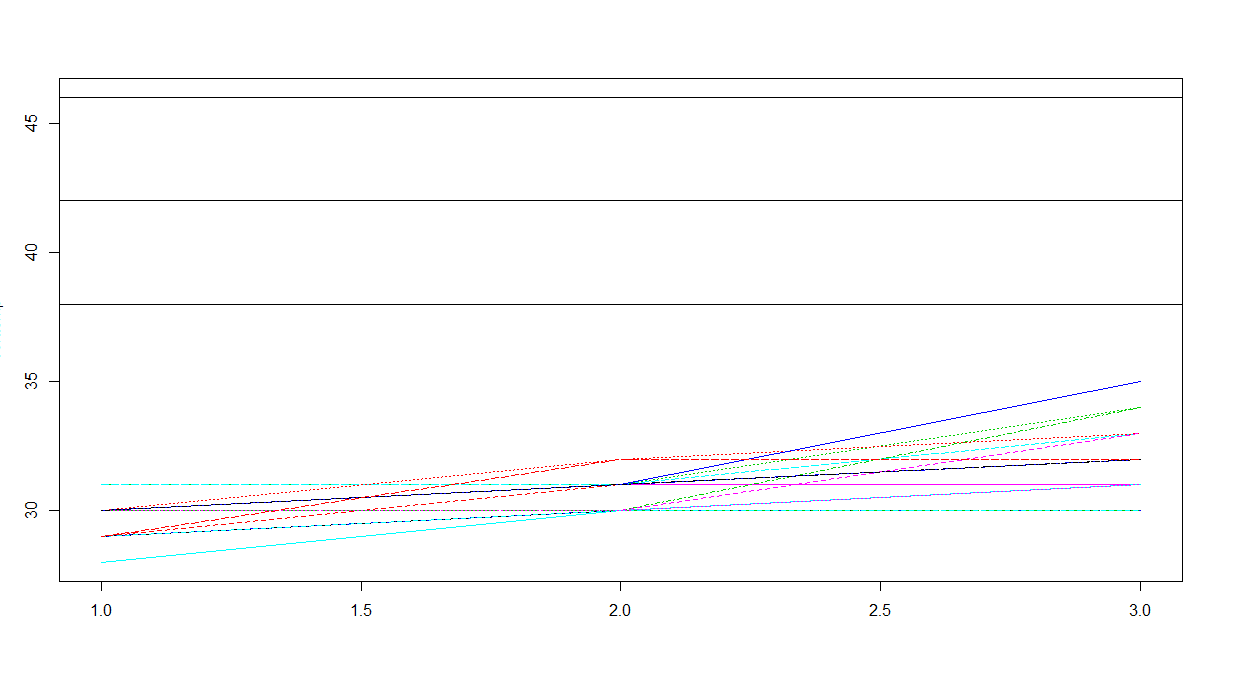
\includegraphics[width=0.9\linewidth]{byrowmat.png}
\end{figure}
\end{frame}
\begin{frame}
\begin{figure}
\centering
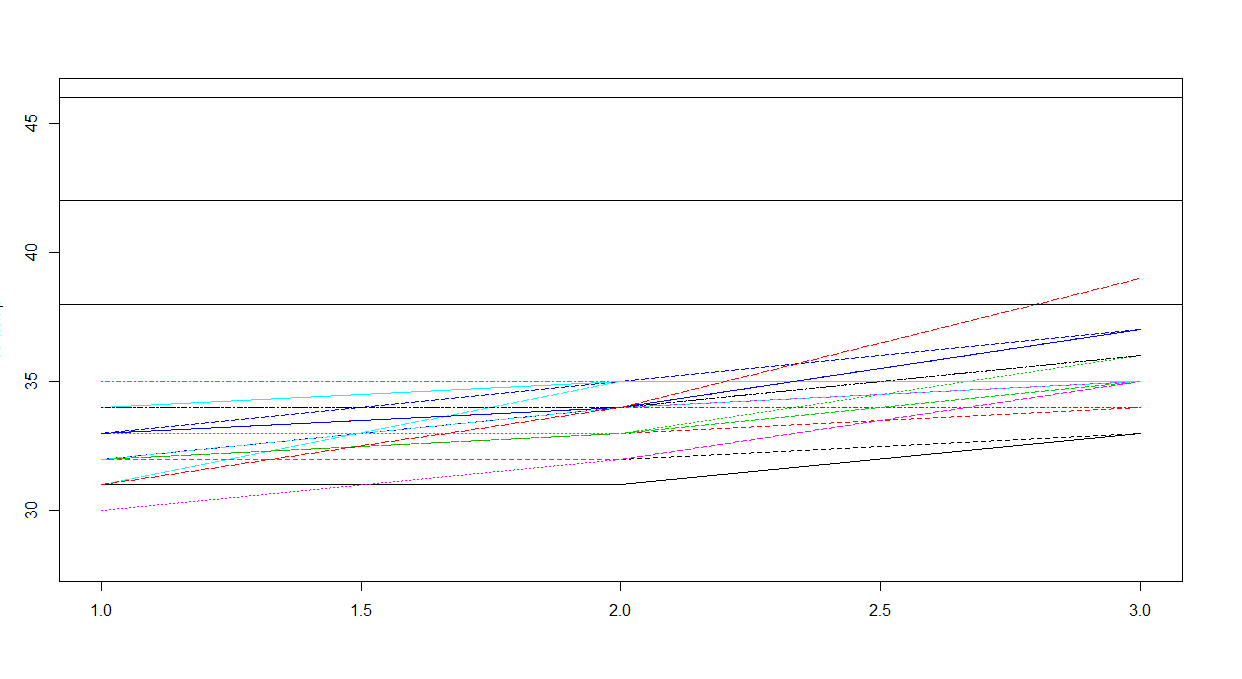
\includegraphics[width=0.9\linewidth]{bycolmat.png}
\end{figure}
\end{frame}
\begin{frame}
\begin{figure}
\centering
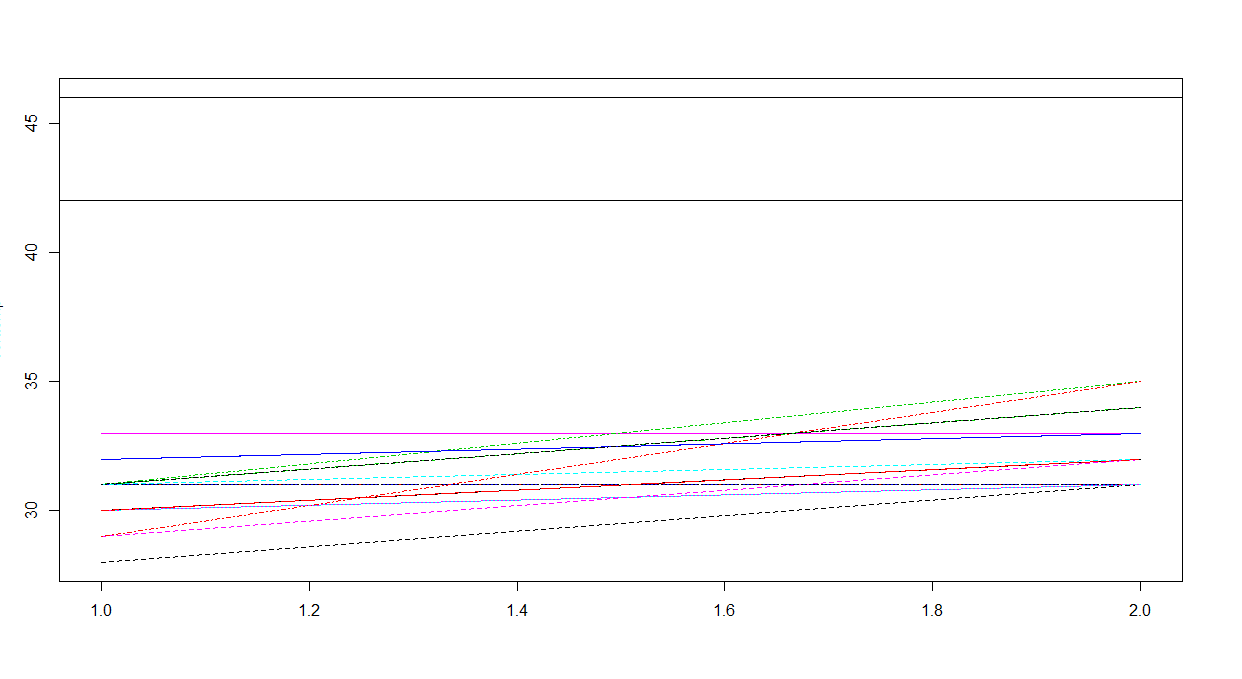
\includegraphics[width=0.9\linewidth]{twoslices.png}
\caption{$t=2$,$k_{\min}=4,k_{\max}=6$, shuffled by row}
\end{figure}
\end{frame}
\begin{frame}
\begin{figure}
\centering
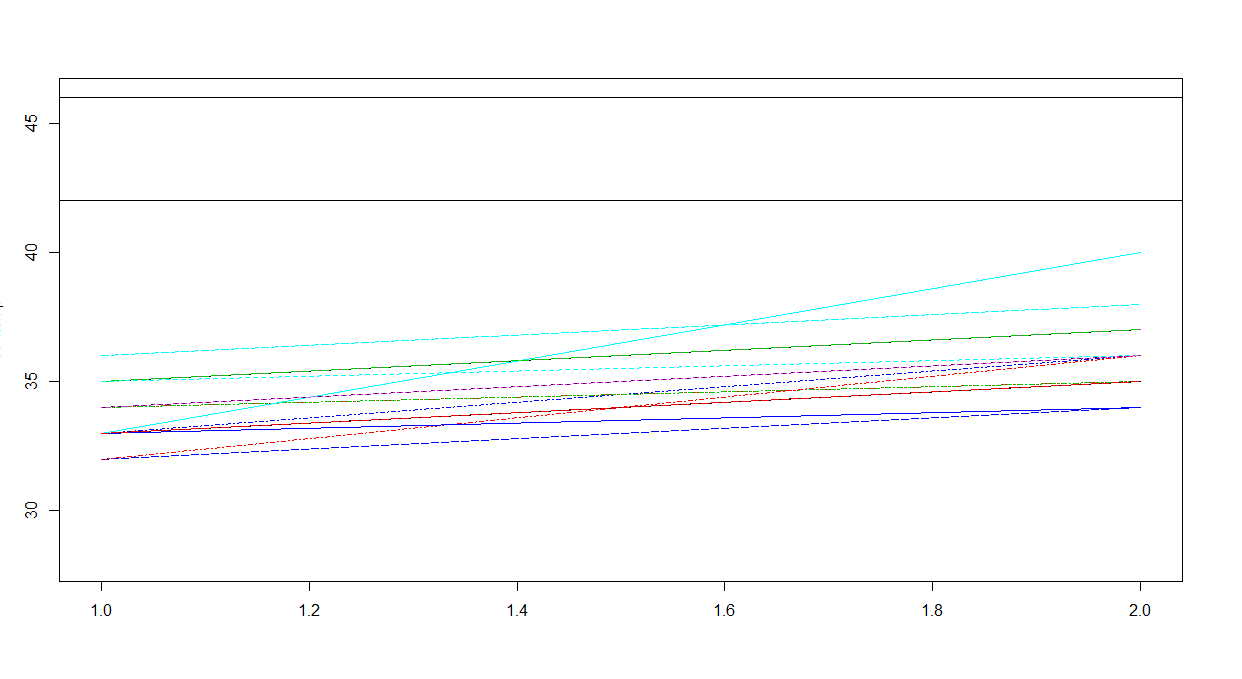
\includegraphics[width=0.9\linewidth]{twoslicesbycolumn.png}
\caption{$t=2$,$k_{\min}=4,k_{\max}=6$, shuffled by column}
\end{figure}
\end{frame}


\end{document}
